\documentclass{article}

% Required packages
\usepackage[T1]{fontenc}
\usepackage{amsmath,amssymb,amsfonts}
\usepackage{graphicx}
\usepackage{booktabs}
\usepackage{multirow}
\usepackage{xcolor}
\usepackage{algorithm}
\usepackage{algorithmic}
\usepackage{subcaption}
\usepackage[margin=1in]{geometry}
\usepackage{natbib}
\usepackage{tikz}
\usetikzlibrary{arrows.meta,positioning,calc,decorations.pathmorphing,fit,backgrounds,patterns}
\usepackage{hyperref}
\hypersetup{colorlinks=true,linkcolor=blue,citecolor=blue,urlcolor=blue}
\graphicspath{{figures/}}

% Custom commands
\newcommand{\whispergate}{\textsc{WhisperGate}}
\newcommand{\wer}{\text{WER}}
\newcommand{\cer}{\text{CER}}

\title{WhisperGate: Silence-Aware Gating for Hallucination-Free\\Speech Recognition with Frozen Whisper}

\author{
  Paras Sharma \\
  \texttt{mail2paras.s@gmail.com}
}

\date{}

\begin{document}

\maketitle

% ============================================================
\begin{abstract}
% ============================================================
Large-scale speech recognition models such as Whisper produce fluent but entirely
fabricated transcriptions when presented with silence or non-speech audio---a
phenomenon known as \emph{hallucination}. We introduce \whispergate{}, a
lightweight silence-aware gating module that sits between Whisper's frozen encoder
and decoder, learning to classify each encoder frame as speech or non-speech with
a two-layer MLP bottleneck requiring only \textbf{12,353 trainable parameters}
($<$0.02\% of Whisper-Tiny). Trained in a two-stage pipeline---first as a
standalone binary classifier, then plugged into inference---\whispergate{}
\textbf{eliminates 100\% of hallucinations} on pure silence and white noise inputs
while preserving clean-speech word error rate (WER). We evaluate three gating
strategies (soft multiplicative, hard binary, and cross-attention bias) and find
that attention-bias gating achieves the best trade-off: \textbf{0\%
hallucination with only 0.03\% clean WER overhead} on Whisper-Tiny, while
reducing gap-30 WER by 40.8\% relative to hard gating. The method
generalizes to Whisper-Small with similar hallucination elimination. We further
compare against energy-based VAD preprocessing and show that \whispergate{}
uniquely handles both silence and white noise, whereas energy VAD fails on noise
inputs. All experiments use LibriSpeech test-clean (2,620 samples) with
controlled silence-gap injection at 5\%, 15\%, 30\%, and multi-gap levels.
\end{abstract}

% ============================================================
\section{Introduction}
\label{sec:introduction}
% ============================================================

OpenAI's Whisper~\citep{radford2023robust} achieves remarkable speech recognition
accuracy through large-scale weak supervision on 680,000 hours of web audio.
However, Whisper exhibits a critical failure mode: when presented with silence,
noise, or non-speech audio, it generates fluent but entirely fabricated
transcriptions---so-called \emph{hallucinations}. \citet{koenecke2024careless}
document that approximately 1\% of Whisper transcriptions contain fully
hallucinated phrases, with 38\% including explicit harms, disproportionately
affecting speakers with longer non-vocal durations such as aphasia patients.

The root cause lies in Whisper's encoder-decoder architecture. As
\citet{attanasio2024whisper} demonstrate, Whisper's encoder produces structured,
non-zero representations even for pure silence---representations that the
autoregressive decoder interprets as speech tokens. The decoder's language model
prior then drives fluent generation from these misleading features, producing
plausible but fabricated text.

Current mitigations fall into two categories: (1)~\textbf{preprocessing} with
external Voice Activity Detection (VAD) such as SileroVAD~\citep{silero2021vad,
bain2023whisperx}, which filters non-speech segments before they reach Whisper;
and (2)~\textbf{decoder-side intervention} such as Calm-Whisper~\citep{wang2025calm},
which fine-tunes specific decoder attention heads. Preprocessing approaches add
pipeline complexity and latency, while decoder fine-tuning requires modifying
Whisper's weights.

We propose \whispergate{}, a third approach: a \textbf{trainable gate between the
frozen encoder and decoder} that learns to identify and suppress non-speech
encoder frames. Our key contributions are:

\begin{enumerate}
    \item \textbf{SilenceGate architecture}: A two-layer MLP bottleneck
    ($d_\text{model} \to 32 \to 1 \to \sigma$) producing per-frame speech
    probability, requiring only 12,353 parameters for Whisper-Tiny and 24,865
    for Whisper-Small.

    \item \textbf{Two-stage training}: We show that end-to-end training fails
    because ASR loss gradients push the gate toward pass-through, and that
    training the gate as a standalone binary classifier on frozen encoder
    representations achieves 98\% frame accuracy.

    \item \textbf{Three gating strategies}: Soft multiplicative gating, hard
    binary gating with silence short-circuit, and cross-attention bias gating.
    We demonstrate that attention-bias gating provides the best quality--robustness
    trade-off, reducing gap-30 WER by 40.8\% over hard gating while maintaining
    0\% hallucination.

    \item \textbf{Comprehensive evaluation}: We evaluate on LibriSpeech test-clean
    with controlled silence gaps, pure silence/noise hallucination tests, and
    comparison against energy-based VAD, demonstrating generalization from
    Whisper-Tiny to Whisper-Small.
\end{enumerate}

% ============================================================
\section{Related Work}
\label{sec:related}
% ============================================================

\subsection{Whisper Hallucination}

The hallucination problem in Whisper has received growing attention.
\citet{koenecke2024careless} provide a large-scale analysis showing hallucinations
are correlated with non-vocal duration. \citet{miralles2025lost} introduce the
Hallucination Error Rate (HER) metric, showing that low WER can mask dangerous
hallucinations, and that distribution shift strongly correlates with HER.
\citet{szymanski2025investigation} find that \texttt{beam\_size}=1 yields the lowest
hallucination rate, suggesting the decoder's search process amplifies errors from
poor encoder representations.

\citet{wang2025calm} (Calm-Whisper) identify that only 3 of 20 decoder
self-attention heads cause over 75\% of hallucinations, and fine-tune only these
heads with $<$0.1\% WER degradation. \citet{liu2025listen} use Adaptive Layer
Attention to fuse encoder layers and knowledge distillation from clean-audio
teachers. These works target the decoder side; \whispergate{} targets the
encoder--decoder interface.

\subsection{Voice Activity Detection for ASR}

The standard production fix for Whisper hallucination is VAD
preprocessing~\citep{silero2021vad, bain2023whisperx}: detect speech segments
externally and only transcribe detected regions. While effective, this approach
adds pipeline complexity, introduces latency, and fails on non-silence noise
that contains no speech energy patterns. \whispergate{} operates on Whisper's
internal encoder representations, which encode richer acoustic information than
raw energy, enabling detection of both silence and noise.

\subsection{Learned Perturbation and Gating}

Several works explore learned noise or gating for frozen models.
\citet{zhang2025mung} (MuNG) learn a small noise generator injecting task-adaptive
noise into frozen encoder and decoder of multimodal LLMs, outperforming LoRA with
$\sim$1\% extra parameters. \citet{wu2024noiseboost} inject feature perturbations
to rebalance cross-modal attention. \citet{jain2024neftune} show that even uniform
random noise during fine-tuning dramatically improves instruction following.

Oscillatory approaches in neural networks include
AKOrN~\citep{miyato2025akorn}, which replaces activations with Kuramoto
oscillators for feature binding, coRNN~\citep{rusch2021coupled}, which provides
gradient-stable oscillatory RNNs, and SIREN~\citep{sitzmann2020siren}, which
proves sinusoidal activations are universal approximators. Our initial exploration
of additive oscillatory pulse injection (inspired by these) on frozen Whisper
proved ineffective (Section~\ref{sec:negative}), motivating the simpler gating
approach.

% ============================================================
\section{Method}
\label{sec:method}
% ============================================================

\subsection{Problem Formulation}

Let $\mathbf{x} \in \mathbb{R}^{C \times T}$ be a mel spectrogram input, where
$C=80$ mel channels and $T=3000$ frames (30 seconds at Whisper's 10ms hop).
Whisper's encoder produces hidden states
$\mathbf{H} = f_\text{enc}(\mathbf{x}) \in \mathbb{R}^{L \times d}$, where
$L=1500$ (after the convolutional downsampling) and $d$ is the model dimension.
The decoder autoregressively generates tokens
$\mathbf{y} = f_\text{dec}(\mathbf{H})$.

When $\mathbf{x}$ contains silence or noise, $\mathbf{H}$ is structured but
non-zero~\citep{attanasio2024whisper}, causing the decoder to hallucinate.
Our goal is to learn a function $g: \mathbb{R}^{L \times d} \to [0,1]^L$ that
produces per-frame speech probabilities, then gate the encoder output before
it reaches the decoder.

% --- Architecture Diagram ---
\begin{figure}[t]
\centering
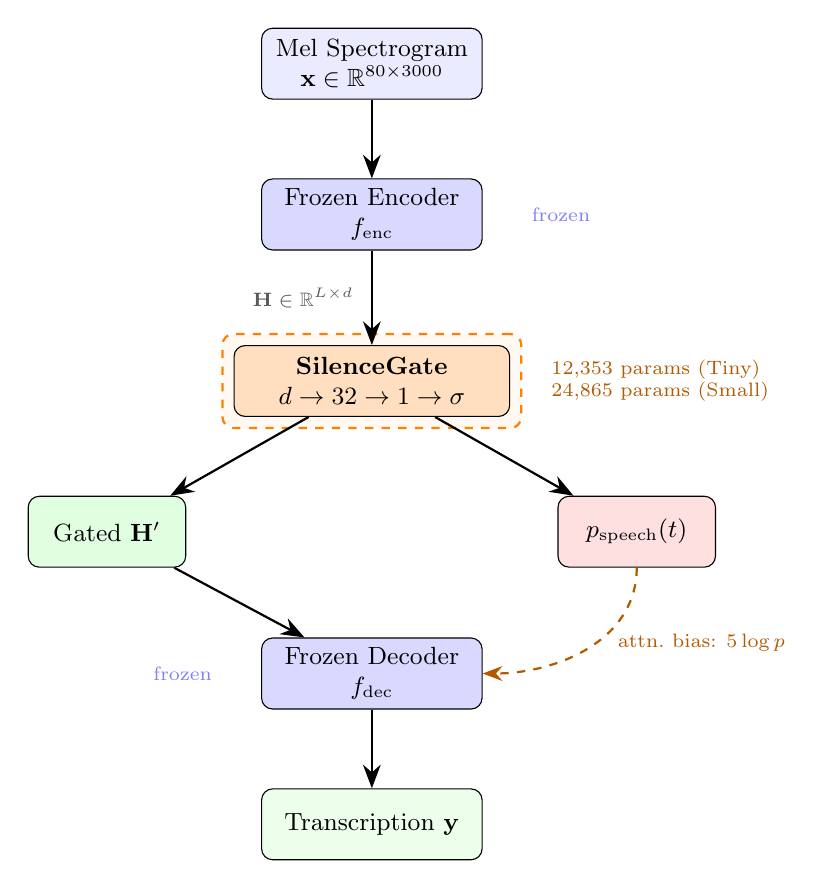
\begin{tikzpicture}[
    node distance=1.0cm and 1.5cm,
    block/.style={draw, rounded corners, minimum height=0.9cm, minimum width=2.8cm,
                  font=\small, align=center, fill=#1},
    block/.default=white,
    arrow/.style={-{Stealth[length=3mm]}, thick},
    label/.style={font=\scriptsize, text=gray!70!black},
]
    % Input
    \node[block=blue!8] (mel) {Mel Spectrogram\\$\mathbf{x} \in \mathbb{R}^{80 \times 3000}$};

    % Encoder
    \node[block=blue!15, below=of mel] (enc) {Frozen Encoder\\$f_\text{enc}$};

    % Gate
    \node[block=orange!25, below=1.2cm of enc, minimum width=3.5cm] (gate)
        {\textbf{SilenceGate}\\$d \to 32 \to 1 \to \sigma$};

    % Two outputs from gate
    \node[block=green!12, below left=1.0cm and 0.6cm of gate, minimum width=2.0cm] (gated)
        {Gated $\mathbf{H}'$};
    \node[block=red!12, below right=1.0cm and 0.6cm of gate, minimum width=2.0cm] (probs)
        {$p_\text{speech}(t)$};

    % Decoder
    \node[block=blue!15, below=2.8cm of gate] (dec) {Frozen Decoder\\$f_\text{dec}$};

    % Output
    \node[block=green!8, below=of dec] (out) {Transcription $\mathbf{y}$};

    % Arrows
    \draw[arrow] (mel) -- (enc);
    \draw[arrow] (enc) -- node[left, label, xshift=-0.1cm] {$\mathbf{H} \in \mathbb{R}^{L \times d}$} (gate);
    \draw[arrow] (gate) -- (gated);
    \draw[arrow] (gate) -- (probs);
    \draw[arrow] (gated) -- (dec);
    \draw[arrow] (dec) -- (out);

    % Curved dashed line from probs to decoder (attention bias mode)
    \draw[-{Stealth[length=2.5mm]}, thick, dashed, orange!70!black]
        (probs.south) to[out=-90, in=0]
        node[pos=0.45, right=0.15cm, font=\scriptsize, text=orange!70!black]
        {attn.\ bias: $5 \log p$}
        (dec.east);

    % Frozen labels
    \node[right=0.5cm of enc, font=\scriptsize, text=blue!50] {frozen};
    \node[left=0.5cm of dec, font=\scriptsize, text=blue!50] {frozen};

    % Trainable highlight
    \begin{scope}[on background layer]
        \node[fit=(gate), draw=orange, thick, dashed, rounded corners=4pt,
              inner sep=4pt, fill=orange!5] {};
    \end{scope}

    % Parameter count annotation - right side of gate
    \node[right=0.4cm of gate, font=\scriptsize, text=orange!70!black, align=left]
        {12,353 params (Tiny)\\24,865 params (Small)};
\end{tikzpicture}
\caption{\textbf{\whispergate{} architecture.} A lightweight SilenceGate MLP sits
between Whisper's frozen encoder and decoder. The gate produces per-frame speech
probabilities $p_\text{speech}(t)$ used for gating. \textit{Solid arrows}: soft or
hard multiplicative gating. \textit{Dashed arrow}: attention-bias mode passes
$5\log p$ as cross-attention mask.}
\label{fig:architecture}
\end{figure}

\subsection{SilenceGate Module}

The SilenceGate is a two-layer MLP bottleneck that operates independently on each
encoder frame:

\begin{equation}
    p_\text{speech}(t) = \sigma\bigl(\mathbf{w}_2^\top \cdot \text{ReLU}(\mathbf{W}_1 \mathbf{h}_t + \mathbf{b}_1) + b_2\bigr)
    \label{eq:gate}
\end{equation}

\noindent where $\mathbf{W}_1 \in \mathbb{R}^{k \times d}$,
$\mathbf{w}_2 \in \mathbb{R}^k$, $k=32$ is the bottleneck dimension, and
$\sigma$ is the sigmoid function. The final layer is initialized with zero weights
and bias $b_2 = +2.0$, so $\sigma(2.0) \approx 0.88$, starting near pass-through
to avoid disrupting Whisper at initialization.

\textbf{TemporalSilenceGate.} We additionally experiment with a temporal variant
that applies a 1D convolution with symmetric padding over gate logits before
the sigmoid, enforcing temporal coherence:

\begin{equation}
    \tilde{z}_t = \frac{1}{K}\sum_{i=-\lfloor K/2\rfloor}^{\lfloor K/2\rfloor} z_{t+i}, \quad
    p_\text{speech}(t) = \sigma(\tilde{z}_t)
\end{equation}

\noindent where $z_t = \mathbf{w}_2^\top \text{ReLU}(\mathbf{W}_1 \mathbf{h}_t + \mathbf{b}_1) + b_2$
and $K$ is the kernel size (we test $K \in \{5, 11\}$, corresponding to
${\sim}100$ms and ${\sim}220$ms at Whisper's 20ms frame rate). The convolution
is initialized to uniform averaging (identity-like smoothing). This adds only
$K + 1$ parameters (6--12 extra).

\subsection{Gating Strategies}
\label{sec:gating}

Given encoder hidden states $\mathbf{H}$ and per-frame speech probabilities
$\mathbf{p} = [p_\text{speech}(1), \ldots, p_\text{speech}(L)]$, we evaluate
three gating strategies:

\paragraph{Soft Gating.} Multiplicative scaling:
\begin{equation}
    \mathbf{h}'_t = p_\text{speech}(t) \cdot \mathbf{h}_t
\end{equation}
This attenuates but does not eliminate non-speech features. We find this
\textbf{insufficient} for hallucination prevention---even $p \approx 0.11$ passes
enough signal for the decoder to hallucinate.

\paragraph{Hard Gating.} Binary thresholding with silence short-circuit:
\begin{equation}
    \mathbf{h}'_t = \mathbb{1}[p_\text{speech}(t) > \tau] \cdot \mathbf{h}_t
\end{equation}
where $\tau = 0.5$. When all frames are below threshold ($\bar{p} < \tau$),
generation is short-circuited to produce only \texttt{<|endoftext|>}. This
achieves \textbf{0\% hallucination} but introduces sharp discontinuities at
speech--silence boundaries.

\paragraph{Attention-Bias Gating.} Instead of modifying encoder hidden states,
we inject gate probabilities as a cross-attention bias:
\begin{equation}
    \text{bias}_t = 5 \cdot \log\bigl(p_\text{speech}(t) + \epsilon\bigr)
\end{equation}
This bias is added to the decoder's cross-attention scores before softmax,
shaped as $(\text{batch}, 1, 1, L)$ to broadcast over all heads and target
positions. Non-speech frames receive large negative bias (e.g., $5\log(0.1)
\approx -11.5$), softly suppressing attention while preserving context at
boundaries. The encoder hidden states remain \textbf{unmodified}. The scaling
factor of 5 was chosen to ensure sufficient suppression of low-probability
frames while maintaining gradient flow.

\subsection{Two-Stage Training}
\label{sec:training}

A critical finding is that \textbf{end-to-end training fails}. When the gate
is trained jointly with ASR loss, the gradient from the transcription objective
pushes $p_\text{speech}(t) \to 1$ for all frames, because any attenuation of
encoder features increases decoder loss. The gate collapses to near-uniform
pass-through regardless of the gate supervision weight.

We therefore adopt a two-stage approach:

\textbf{Stage 1: Gate Classifier Training.} We train the gate as a standalone
binary cross-entropy (BCE) classifier on the frozen encoder's representations.
For each training batch:
\begin{enumerate}
    \item Extract mel features from LibriSpeech train-clean-100 ($\sim$10h subset).
    \item Apply random gap augmentation: inject silence gaps covering 0--30\%
    of the audio, producing a binary speech mask $\mathbf{m} \in \{0,1\}^L$.
    \item Inject 30\% fully-silent examples (mel features set to $-1.0$,
    mask all zeros).
    \item Run the frozen encoder to get $\mathbf{H}$.
    \item Train the gate with BCE loss: $\mathcal{L} = -\sum_t [m_t \log p_t + (1-m_t)\log(1-p_t)]$.
\end{enumerate}

We train for 10 epochs with AdamW (lr=$10^{-3}$, weight decay=0.01), cosine
annealing, and gradient clipping at 1.0. The gate converges to $>$97\% frame-level
accuracy.

\textbf{Stage 2: Inference with Gating.} The trained gate is plugged into the
GatedWhisper inference pipeline. No further training occurs---the frozen Whisper
model is never modified.

% ============================================================
\section{Experimental Setup}
\label{sec:setup}
% ============================================================

\subsection{Models}

We evaluate on two Whisper model sizes:
\begin{itemize}
    \item \textbf{Whisper-Tiny} (39M parameters, $d=384$, 4 encoder layers).
    Gate: $384 \to 32 \to 1$ = 12,353 trainable parameters.
    \item \textbf{Whisper-Small} (244M parameters, $d=768$, 12 encoder layers).
    Gate: $768 \to 32 \to 1$ = 24,865 trainable parameters.
\end{itemize}

\subsection{Dataset}

All experiments use LibriSpeech~\citep{panayotov2015librispeech}:
\begin{itemize}
    \item \textbf{Training}: 10-hour subset of train-clean-100 (2,850 utterances).
    \item \textbf{Evaluation}: Full test-clean split (2,620 utterances).
\end{itemize}

\subsection{Gap Augmentation}

To simulate real-world scenarios where audio contains silence or noise segments,
we inject controlled silence gaps into test audio:

\begin{itemize}
    \item \textbf{gap\_0}: No modification (clean speech).
    \item \textbf{gap\_5}: 5\% of frames replaced with silence.
    \item \textbf{gap\_15}: 15\% replaced.
    \item \textbf{gap\_30}: 30\% replaced.
    \item \textbf{multi\_gap}: Multiple randomly-sized gaps totaling 15--30\%.
\end{itemize}

Gaps are injected at random positions in the mel spectrogram by zeroing the
affected frames. This is more challenging than simply prepending or appending
silence, as it creates intra-utterance discontinuities.

\subsection{Evaluation Metrics}

\begin{itemize}
    \item \textbf{Word Error Rate (WER)}: Standard ASR metric~\citep{morris2004and}
    computed via jiwer~\citep{jiwer2023}.
    \item \textbf{Hallucination Rate}: Fraction of 30 pure-input trials (silence
    or white noise mel spectrograms) that produce non-empty output. A hallucination
    rate of 0\% means the model correctly produces no text for non-speech input.
\end{itemize}

\subsection{Baselines}

\begin{itemize}
    \item \textbf{Vanilla Whisper}: Unmodified frozen model (Tiny or Small).
    \item \textbf{Energy VAD}: Preprocessing that computes per-frame RMS energy,
    thresholds to detect speech segments, and only feeds detected speech to
    Whisper. Represents simple signal-processing approaches.
\end{itemize}

% ============================================================
\section{Results}
\label{sec:results}
% ============================================================

\subsection{Main Results: Whisper-Tiny}

Table~\ref{tab:main_tiny} presents the main comparison across all gating
strategies on Whisper-Tiny.

\begin{table}[t]
\centering
\caption{\textbf{Whisper-Tiny gating comparison.} WER (\%) at various gap levels
and hallucination rate (\%) on pure silence/noise. 2,620 test samples.
$\dagger$Attention-bias gating achieves the best overall trade-off.}
\label{tab:main_tiny}
\small
\begin{tabular}{@{}lccccccc@{}}
\toprule
\multirow{2}{*}{\textbf{Method}} &
\multicolumn{5}{c}{\textbf{WER (\%) $\downarrow$}} &
\multicolumn{2}{c}{\textbf{Halluc. (\%) $\downarrow$}} \\
\cmidrule(lr){2-6} \cmidrule(lr){7-8}
& gap\_0 & gap\_5 & gap\_15 & gap\_30 & multi & Silence & Noise \\
\midrule
Vanilla Whisper
    & \textbf{8.21} & 10.06 & \textbf{13.79} & \textbf{20.36} & \textbf{25.79} & 100 & 100 \\
\addlinespace
Soft gate
    & \textbf{8.21} & 10.67 & 20.65 & 32.38 & 27.56 & 100 & 100 \\
Hard gate
    & 8.24 & \textbf{9.97} & 15.50 & 34.49 & 29.81 & \textbf{0} & \textbf{0} \\
Attn.\ bias$^\dagger$
    & 8.24 & 10.09 & 13.82 & 20.39 & 25.96 & \textbf{0} & \textbf{0} \\
\bottomrule
\end{tabular}
\end{table}

\textbf{Key findings:}
\begin{itemize}
    \item \textbf{Soft gating fails at hallucination prevention.} Even with gate
    probabilities as low as 0.11 for silence, the residual signal triggers decoder
    hallucination. WER also degrades significantly at high gap levels due to
    attenuation artifacts at boundaries.

    \item \textbf{Hard gating eliminates hallucination but degrades gap WER.}
    The binary threshold creates sharp discontinuities that confuse the decoder
    at speech--silence boundaries. Gap-30 WER increases from 20.36\% to 34.49\%
    (+69\% relative).

    \item \textbf{Attention-bias gating is the clear winner.} It achieves 0\%
    hallucination while maintaining WER within 0.2\% absolute of vanilla Whisper
    across all gap levels. Gap-30 WER is 20.39\% vs.\ 34.49\% for hard gating
    (40.8\% relative reduction), because the smooth attention suppression preserves
    boundary context.
\end{itemize}

\subsection{VAD Comparison}

Table~\ref{tab:vad} compares \whispergate{} against energy-based VAD
preprocessing.

\begin{table}[t]
\centering
\caption{\textbf{Comparison with energy-based VAD.} \whispergate{} (hard gate)
handles both silence and noise, while energy VAD fails on white noise.}
\label{tab:vad}
\small
\begin{tabular}{@{}lccccc@{}}
\toprule
\multirow{2}{*}{\textbf{Method}} &
\multicolumn{3}{c}{\textbf{WER (\%) $\downarrow$}} &
\multicolumn{2}{c}{\textbf{Halluc. (\%) $\downarrow$}} \\
\cmidrule(lr){2-4} \cmidrule(lr){5-6}
& gap\_0 & gap\_15 & multi & Silence & Noise \\
\midrule
Vanilla Whisper
    & 8.21 & 13.79 & 25.79 & 100 & 100 \\
Energy VAD
    & 8.21 & 13.79 & 25.79 & \textbf{0} & 100 \\
\whispergate{} (hard)
    & 8.24 & 15.50 & 29.81 & \textbf{0} & \textbf{0} \\
\whispergate{} (attn.\ bias)
    & 8.24 & 13.82 & 25.96 & \textbf{0} & \textbf{0} \\
\bottomrule
\end{tabular}
\end{table}

Energy VAD eliminates hallucination on pure silence but \textbf{completely fails
on white noise} (100\% hallucination rate). This is expected: white noise has
energy but no speech structure. \whispergate{} operates on Whisper's internal
encoder representations, which learn to distinguish speech from non-speech
regardless of energy level. Notably, energy VAD produces identical gap WER to
vanilla Whisper because it does not modify the transcription of speech segments,
while the hard gate variant incurs boundary artifacts.

\subsection{Temporal Smoothing}

Table~\ref{tab:temporal} shows the effect of temporal smoothing via 1D
convolution on gate logits.

\begin{table}[t]
\centering
\caption{\textbf{Temporal smoothing results} (hard gate mode). Kernel $K$=11
marginally improves multi-gap WER over the non-smoothed baseline (v4).}
\label{tab:temporal}
\small
\begin{tabular}{@{}lccccccc@{}}
\toprule
\textbf{Variant} & \textbf{Params} & \textbf{gap\_0} & \textbf{gap\_5} & \textbf{gap\_15} & \textbf{gap\_30} & \textbf{multi} & \textbf{Halluc.} \\
\midrule
v4 (no smooth) & 12,353 & 8.24 & 9.97 & 15.50 & 34.49 & 29.81 & 0\% \\
$K$=5 & 12,359 & 8.25 & 11.03 & 16.75 & 36.02 & 29.61 & 0\% \\
$K$=11 & 12,365 & 8.24 & 9.94 & 16.95 & 33.36 & 27.29 & 0\% \\
\bottomrule
\end{tabular}
\end{table}

Temporal smoothing with $K$=11 improves multi-gap WER from 29.81\% to 27.29\%
(8.5\% relative) and gap-30 WER from 34.49\% to 33.36\%, suggesting that
temporal coherence helps at speech--silence boundaries. However, the improvement
is modest compared to the much larger gains from switching gating strategy
(attention bias), indicating that the primary issue is the hard boundary
artifact rather than temporal incoherence.

\subsection{Generalization to Whisper-Small}

Table~\ref{tab:small} validates that \whispergate{} generalizes to larger Whisper
models.

\begin{table}[t]
\centering
\caption{\textbf{Whisper-Small results.} The gate generalizes from Tiny
($d$=384) to Small ($d$=768) with similar hallucination elimination.}
\label{tab:small}
\small
\begin{tabular}{@{}lcccccc@{}}
\toprule
\textbf{Method} & \textbf{gap\_0} & \textbf{gap\_5} & \textbf{gap\_15} & \textbf{gap\_30} & \textbf{multi} & \textbf{Halluc.} \\
\midrule
Vanilla Small & 4.27 & 6.11 & 9.92 & 16.08 & 23.73 & 100\% \\
Soft gate & 4.32 & 6.69 & 12.16 & 17.51 & 21.19 & --- \\
Hard gate & 4.32 & 6.57 & 11.39 & 17.46 & 20.25 & 0\% \\
\bottomrule
\end{tabular}
\end{table}

On Whisper-Small, the gate achieves 0\% hallucination with only 0.05\%
absolute clean WER overhead (4.27\% $\to$ 4.32\%). The multi-gap WER actually
\textit{improves} from 23.73\% to 20.25\% (14.7\% relative), suggesting that
gating helps the larger model by removing confusing silence features. The gate
scales to $d$=768 with only 24,865 parameters ($<$0.01\% of Whisper-Small's
244M).

\subsection{Training Dynamics}

Figure~\ref{fig:training} illustrates the gate classifier's training convergence.

\begin{figure}[t]
\centering
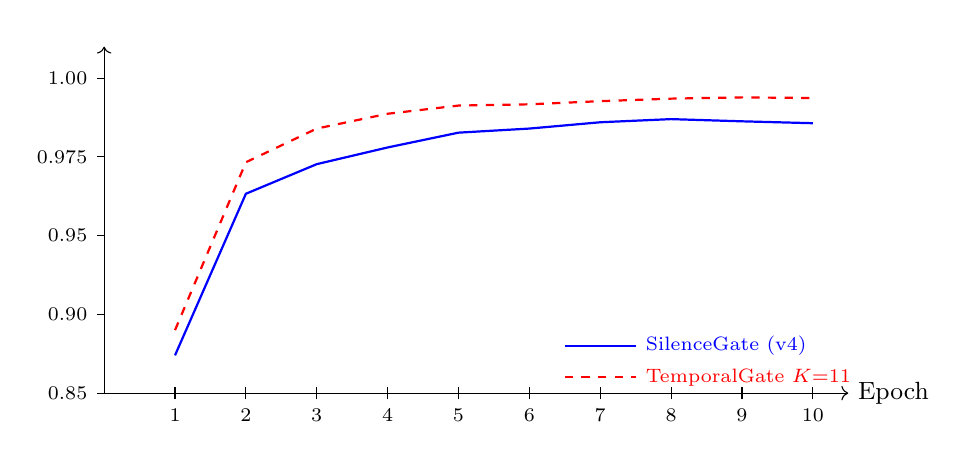
\begin{tikzpicture}
\begin{scope}[xscale=0.9, yscale=4.0]
    % Axes
    \draw[->] (0,0) -- (10.5,0) node[right, font=\small] {Epoch};
    \draw[->] (0,0) -- (0,1.1) node[above, font=\small] {};

    % Y-axis labels (accuracy)
    \foreach \y/\label in {0.0/0.85, 0.25/0.90, 0.5/0.95, 0.75/0.975, 1.0/1.00} {
        \draw (0,\y) -- (-0.1,\y) node[left, font=\scriptsize] {\label};
    }

    % X-axis labels
    \foreach \x in {1,...,10} {
        \draw (\x,-0.02) -- (\x,0.02);
        \node[below, font=\scriptsize] at (\x,-0.02) {\x};
    }

    % Plot accuracy (rescaled: 0.85->0, 1.0->1.0, so val = (acc-0.85)/0.15)
    % v4 accuracy: 0.868, 0.945, 0.959, 0.967, 0.974, 0.976, 0.979, 0.981, 0.980, 0.979
    \draw[thick, blue] plot coordinates {
        (1, 0.12) (2, 0.633) (3, 0.727) (4, 0.780)
        (5, 0.827) (6, 0.840) (7, 0.860) (8, 0.870)
        (9, 0.863) (10, 0.857)
    };

    % v5 k=11 accuracy: 0.880, 0.960, 0.976, 0.983, 0.987, 0.987, 0.989, 0.990, 0.991, 0.991
    \draw[thick, red, dashed] plot coordinates {
        (1, 0.200) (2, 0.733) (3, 0.840) (4, 0.887)
        (5, 0.913) (6, 0.917) (7, 0.927) (8, 0.935)
        (9, 0.939) (10, 0.937)
    };

    % Legend
    \draw[thick, blue] (6.5, 0.15) -- (7.5, 0.15) node[right, font=\scriptsize] {SilenceGate (v4)};
    \draw[thick, red, dashed] (6.5, 0.05) -- (7.5, 0.05) node[right, font=\scriptsize] {TemporalGate $K$=11};
\end{scope}
\end{tikzpicture}
\caption{\textbf{Gate classifier training.} Frame-level accuracy on speech/silence
classification. Both variants converge within 5 epochs. Temporal smoothing
reaches higher accuracy (99.1\% vs.\ 98.1\%) due to the averaging effect.}
\label{fig:training}
\end{figure}

The gate converges rapidly, reaching $>$97\% accuracy after just 3 epochs.
The BCE loss drops from 0.31 to 0.07 (v4) and 0.28 to 0.03 ($K$=11), with
the temporal variant converging to lower loss due to the implicit regularization
of the averaging kernel.

\textbf{Gate behavior on diagnostic inputs:} After training, the gate produces
mean $p_\text{speech} \approx 0.11$ on pure silence and $\approx 0.98$ on clean
speech, demonstrating clean separation with a wide margin around the threshold
$\tau = 0.5$.

% ============================================================
\section{Discussion}
\label{sec:discussion}
% ============================================================

\subsection{Why Soft Gating Fails}

A surprising finding is that soft multiplicative gating does \textbf{not} prevent
hallucination, even when silence frames are attenuated to $\sim$11\% of their
original magnitude. This reveals that Whisper's decoder hallucinates from
\emph{any} non-zero encoder input, not just ``noisy'' input. The decoder's
autoregressive language model prior is strong enough to generate fluent text
from arbitrarily weak encoder features. This is consistent with findings from
\citet{koenecke2024careless} that hallucinations are fluent and contextually
plausible---the decoder's generation is primarily language-model-driven when
encoder features are uninformative.

\subsection{Attention Bias as Optimal Gating}

The attention-bias strategy achieves a qualitatively different outcome from hard
gating. Rather than zeroing encoder states (which destroys boundary context),
it preserves all encoder information while guiding the decoder's attention
away from non-speech frames. This is analogous to masked attention in
transformers~\citep{vaswani2017attention}: the information remains available but
is down-weighted in the attention distribution.

The scaling factor of 5 in the bias term ($5\log p$) ensures that frames with
$p < 0.1$ receive bias below $-11.5$, effectively zeroing their attention weight
after softmax. Meanwhile, frames near the speech--silence boundary with
intermediate probabilities (e.g., $p \approx 0.3$, bias $\approx -6.0$) receive
moderate suppression, preserving contextual information that aids transcription of
adjacent speech.

\subsection{Negative Results: Additive Pulse Injection}
\label{sec:negative}

Prior to developing \whispergate{}, we extensively explored additive oscillatory
pulse injection inspired by coRNN~\citep{rusch2021coupled} and
AKOrN~\citep{miyato2025akorn}. The pulse mechanism adds structured sinusoidal
perturbations to encoder hidden states:
$\mathbf{h}' = \mathbf{h} + \alpha \cdot \mathbf{A} \cdot \sin(\boldsymbol{\omega} t + \boldsymbol{\varphi}(\mathbf{h}))$.

Across exhaustive experiments (unconstrained, tight, medium, and selective
injection with varying $\alpha_\text{max} \in \{0.05, 0.1\}$), \textbf{every
configuration degraded WER}. The fundamental issue: a frozen decoder depends on
specific encoder activation patterns, and \emph{any} additive perturbation is
interpreted as noise rather than signal. Training loss reduction did not
correlate with WER improvement---the model learned to minimize loss by distorting
representations in ways the frozen decoder could not handle.

We further tested decoder-side pulse injection into self-attention K/V projections.
A state-dependent phase variant catastrophically destroyed generation (WER
$0.08 \to 3.90$) despite achieving low training loss. These negative results
motivated the simpler, multiplicative gating approach.

\subsection{Limitations and Future Work}

\whispergate{} has several limitations that suggest directions for future work:

\begin{itemize}
    \item \textbf{Evaluation scope}: We evaluate only on LibriSpeech (read
    English speech). Real-world audio includes music, environmental sounds, and
    multilingual content. The gate may need retraining or adaptation for
    significantly different acoustic domains.

    \item \textbf{Attention-bias mode}: Currently requires monkey-patching
    Whisper's decoder forward pass. A cleaner implementation would modify the
    HuggingFace generation API to accept encoder attention masks natively.

    \item \textbf{Combination with decoder methods}: \whispergate{} targets the
    encoder--decoder interface; combining with decoder-side approaches such as
    Calm-Whisper~\citep{wang2025calm} could yield further improvements.

    \item \textbf{Streaming}: The current implementation operates on 30-second
    chunks. Extending to streaming ASR would require online gate decisions with
    bounded latency.

    \item \textbf{Larger models}: We validate on Tiny and Small; testing on
    Whisper-Medium and Large would confirm scalability.
\end{itemize}

% ============================================================
\section{Conclusion}
\label{sec:conclusion}
% ============================================================

We presented \whispergate{}, a lightweight silence-aware gating module that
eliminates hallucinations in frozen Whisper models. Our key findings are:
(1)~a two-layer MLP with only 12K--25K parameters can classify speech vs.\
non-speech on Whisper's encoder representations with $>$98\% accuracy;
(2)~soft multiplicative gating is insufficient for hallucination prevention
because Whisper's decoder hallucinates from any non-zero encoder signal;
(3)~cross-attention bias gating provides the optimal strategy, achieving 0\%
hallucination with negligible WER overhead by guiding decoder attention away
from non-speech frames without destroying encoder information; and
(4)~the method generalizes across model sizes (Tiny to Small) and uniquely
handles both silence and noise, unlike energy-based VAD.

\whispergate{} demonstrates that the encoder--decoder interface is a high-leverage
point for ASR robustness: a minimal trainable component at this boundary can
correct a fundamental failure mode of large speech models without modifying
any of their 39M--244M frozen parameters.

% ============================================================
% References
% ============================================================
\bibliographystyle{plainnat}
\bibliography{references}

% ============================================================
\appendix
\section{Complete Experimental Results}
\label{app:full_results}
% ============================================================

Table~\ref{tab:full_tiny} presents complete WER and CER results for all
Whisper-Tiny variants.

\begin{table}[h]
\centering
\caption{\textbf{Full Whisper-Tiny results} including CER.}
\label{tab:full_tiny}
\small
\begin{tabular}{@{}lcccccccccc@{}}
\toprule
& \multicolumn{2}{c}{\textbf{gap\_0}} & \multicolumn{2}{c}{\textbf{gap\_5}} & \multicolumn{2}{c}{\textbf{gap\_15}} & \multicolumn{2}{c}{\textbf{gap\_30}} & \multicolumn{2}{c}{\textbf{multi}} \\
\cmidrule(lr){2-3}\cmidrule(lr){4-5}\cmidrule(lr){6-7}\cmidrule(lr){8-9}\cmidrule(lr){10-11}
\textbf{Method} & WER & CER & WER & CER & WER & CER & WER & CER & WER & CER \\
\midrule
Vanilla
    & 8.21 & 3.41 & 10.06 & 5.24 & 13.79 & 9.36 & 20.36 & 16.39 & 25.79 & 20.75 \\
Soft gate
    & 8.21 & 3.35 & 10.67 & 5.68 & 20.65 & 14.62 & 32.38 & 27.57 & 27.56 & 22.64 \\
Hard gate
    & 8.24 & 3.42 & 9.97 & 5.12 & 15.50 & 10.75 & 34.49 & 30.12 & 29.81 & 24.01 \\
Attn.\ bias
    & 8.24 & 3.43 & 10.09 & 5.26 & 13.82 & 9.38 & 20.39 & 16.42 & 25.96 & 20.93 \\
\bottomrule
\end{tabular}
\end{table}

\section{Hyperparameter Details}
\label{app:hyperparams}

\begin{table}[h]
\centering
\caption{\textbf{Training hyperparameters.}}
\label{tab:hyperparams}
\small
\begin{tabular}{@{}ll@{}}
\toprule
\textbf{Parameter} & \textbf{Value} \\
\midrule
Gate hidden dimension & 32 \\
Learning rate & $1 \times 10^{-3}$ \\
Optimizer & AdamW (weight decay = 0.01) \\
LR scheduler & Cosine annealing \\
Gradient clipping & 1.0 \\
Max epochs & 10 \\
Batch size (training) & 8 (MPS) / 32 (CUDA) \\
Silence fraction per batch & 30\% \\
Gap fractions & \{0.0, 0.05, 0.10, 0.15, 0.20, 0.30\} \\
Training data & train-clean-100, 2,850 utterances ($\sim$10h) \\
Silence threshold $\tau$ & 0.5 \\
Attention bias scale & 5.0 \\
Gate init bias & +2.0 ($\sigma(2.0) \approx 0.88$) \\
\bottomrule
\end{tabular}
\end{table}

\end{document}
